%%%%%%%%%%%%%%%%%%%%%%%%%%%%%%%%%%%%%%%%%%%%%%%%%%%
%% P3: Phenomenology of Particle Physics                         
%%
%% Author:  André Rubbia                   		 
%%
%% Figure 5.1 The angle of the Thomas--Wigner rotation as a function of the boost parameter.
%%
%% This work is licensed under the Creative Commons Attribution 4.0 International License. 
%% To view a copy of this license, visit http://creativecommons.org/licenses/by/4.0/ or 
%% send a letter to Creative Commons, PO Box 1866, Mountain View, CA 94042, USA.
%%
%%%%%%%%%%%%%%%%%%%%%%%%%%%%%%%%%%%%%%%%%%%%%%%%%%%

\documentclass[a4paper,10pt]{article}

\usepackage[T1]{fontenc}
\usepackage[utf8]{inputenc}
\usepackage{lmodern}
\usepackage[labelfont=bf]{caption}
\usepackage{upgreek}

\usepackage{tikz}
\usepackage{pgfplots}
\pgfplotsset{compat=1.17}
\usepgfplotslibrary{ternary}
\usepgfplotslibrary{fillbetween}
\usepgfplotslibrary{external}

\def\d{\mathrm{d}}

\begin{document}

%%%%%%%%%%%%%%%%   FIGURE  %%%%%%%%%%%%%%%%%%%%%%%%%%%%%%
\begin{figure}[htb]
\begin{center}
%\vspace{-0.3cm}
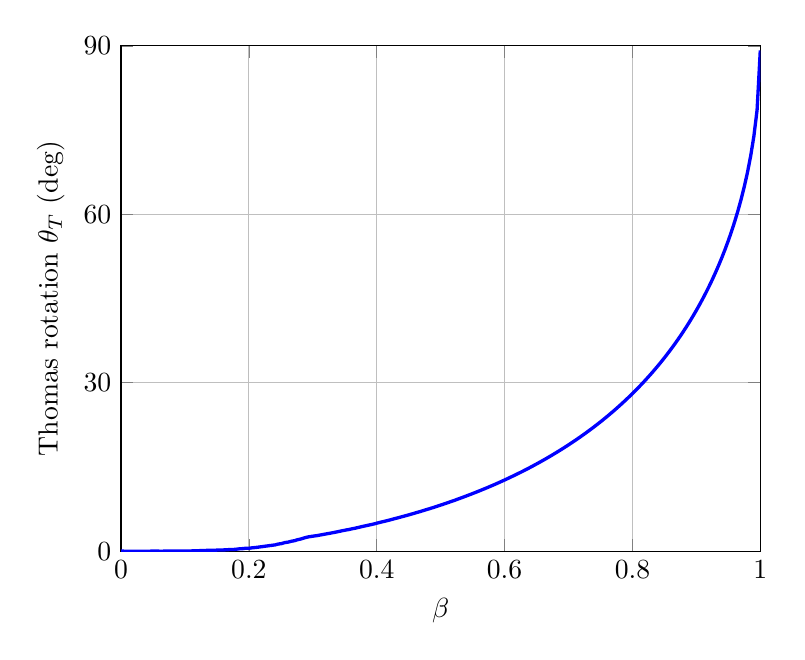
\begin{tikzpicture}[scale=1.]
\begin{axis}[width=0.8\textwidth, height=8cm, xmin=0, xmax=1,
%	xtick={0,0.5,1},
	ytick={0,30,60,90},
	ymin=0, ymax=90,
	xlabel=$\beta$,
	ylabel=Thomas rotation $\theta_T$ (deg),
	xmajorgrids=true,
	ymajorgrids=true,
%	legend entries={$n(x)$,$n'(x)$,$\alpha(x)$},
%	legend pos = outer north east
]
	\addplot[domain=0:1,blue,very thick,samples=200] {acos(2*sqrt(1-x*x)/(2-x*x))};
\end{axis}
\end{tikzpicture}
\caption{The angle of the Thomas--Wigner rotation as a function of the boost parameter $\beta$.}
\end{center}
\end{figure}
%%%%%%%%%%%%%%%%   END FIGURE  %%%%%%%%%%%%%%%%%%%%%%%%%%%%%%
%

\end{document}
